\subsection{Saisir les paramètres de scan 3D}
\begin{enumerate}
    
    \item Sur l'interface d'accueil (voir figure~\ref{fig:accueil}), cliquer sur \textit{CFG Experiment} (7e bouton).
    \item \label{extremums1} Tourner la \textit{roulette de devant} (voir figure~\ref{fig:roulettes}) dans le sens antihoraire jusqu'à atteindre le rebord de l'échantillon, i.e. perdre du signal de fluorescence à l'écran. Il s'agit d'un extremum local mais peut-être pas de l'extremum global.
    \item En se souvenant des observations notées à l'étape~\ref{observations}, tourner un peu la \textit{roulette du dessus}, puis réajuster la \textit{roulette de devant} pour retrouver l'extremum local. Le but est d'avoir la valeur la plus petite possible pour la \textit{roulette de devant}. Les valeurs des roulettes sont affichées comme sur la figure~\ref{fig:roulettes}. Itérer jusqu'à retrouver l'extremum global.
    \item Refaire le même processus, mais en ajustant la \textit{roulette de devant} par rapport à la \textit{roulette de droite}.
    \item \label{extremums2} Une fois la valeur minimale trouvée, cliquer sur \textit{Width LO} (voir figure~\ref{fig:cf}).
        \begin{figure}[H]
        \centering
        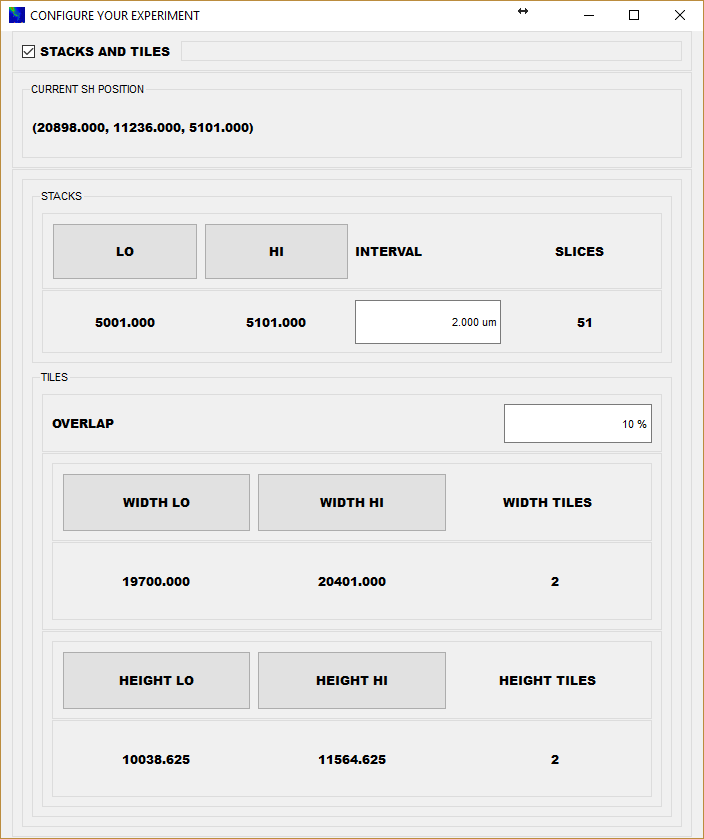
\includegraphics[width=10cm]{cf.png}
        \caption{Fenêtre pop-up de \textit{CFG Experiment}}
        \label{fig:cf}
        \end{figure}
    \item Refaire les étapes~\ref{extremums1} à \ref{extremums2} en suivant l'ordre suivant:
        \begin{itemize}
        \item[$\bullet$] Pour \textit{Width HI}: \textit{roulette de devant} p/r à \textit{roulette de dessus}, puis p/r à \textit{roulette de droite}
        \item[$\bullet$] Pour \textit{Height LO}: \textit{roulette de dessus} p/r à \textit{roulette de devant}, puis p/r à \textit{roulette de droite}
        \item[$\bullet$] Pour \textit{Height HI}: \textit{roulette de dessus} p/r à \textit{roulette de devant}, puis p/r à \textit{roulette de droite}
        \end{itemize}
    *** Les valeurs choisies pour chaque extremum sont gardées en mémoire et affichées sous leur bouton respectif.
    \item Mettre la \textit{roulette de devant} sur la valeur calculée de la façon suivante:
    $$ roulette~de~devant = \frac{valeur~de~Width~HI - valeur~de~Width~LO}{2} + valeur~de~Width~LO $$
    \item Mettre la \textit{roulette du dessus} sur la valeur calculée de la façon suivante:
    $$ roulette~du~dessus = \frac{valeur~de~Height~HI - valeur~de~Height~LO}{2} + valeur~de~Heigth~LO $$
    \item Tourner la \textit{roulette de droite} (voir figure~\ref{fig:roulettes}) dans le sens antihoraire jusqu'à atteindre le rebord de l'échantillon, i.e. perdre du signal de fluorescence à l'écran. Cliquer sur \textit{LO}.
    \item Tourner la \textit{roulette de droite} dans le sens horaire jusqu'à atteindre le rebord de l'échantillon, i.e. perdre du signal de fluorescence à l'écran. Cliquer sur \textit{HI}.
    \item Vérifier que l'intervalle entre chaque stack est de 2.000 um (par défaut) ou plus.
    \item Vérifier que le pourcentage d'overlap est entre 10\% (par défaut) et 20\%.
    \item Cliquer sur X pour fermer la fenêtre.
\end{enumerate}